\documentclass[10pt, addpoints]{exam}
\usepackage[margin=1in]{geometry}
\usepackage{amsmath, amssymb, amsthm, graphicx, hyperref}
\usepackage{enumerate}
\usepackage{color}
\usepackage{graphicx}
\usepackage{epstopdf}
\DeclareGraphicsRule{.tif}{png}{.png}{`convert #1 `dirname #1`/`basename #1 .tif`.png}
\usepackage{multirow, multicol}
\usepackage{pdfpages}
\usepackage{pgfplots}
\usepackage{wrapfig}
\usepackage{stfloats}
\usepackage{tikz}
\usetikzlibrary{arrows.meta}
\usepackage{wasysym}
\firstpageheader{}{}{}
\firstpagefooter{}{}{}
\runningheader{\scalebox{0.25}{\includegraphics{nyu_short_black}}}{}{\tiny Math-UA.120}
\runningfooter{}{\thepage}{}

\newtheorem*{theorem}{Theorem}


%% MC Solution Sheet ----------------------------
\newcommand*\mycirc[1]{%
  \begin{tikzpicture}[baseline=(C.base)]
    \node[draw,circle,inner sep=2pt](C) {#1};
  \end{tikzpicture}}
\renewcommand\choicelabel{\mycirc{\Alph{choice}}}
\CorrectChoiceEmphasis{\color{red}\bfseries} %%% my students were struggling to see the bold text
%% ----------------------------------------------

\printanswers
  
\theoremstyle{definition}
\newtheorem*{definition}{Definition}

\newcommand{\R}{\mathbb{R}}
\newcommand{\E}{\mathbb{E}}
\newcommand{\Z}{\mathbb{Z}}
\newcommand{\N}{\mathbb{N}}
\newcommand{\Q}{\mathbb{Q}}
\newcommand{\proj}{\textbf{proj}}
\newcommand{\curl}{\textrm{curl }}
\renewcommand{\div}{\textrm{ div }}
% For boldface vectors:
\renewcommand{\vec}[1]{\mathbf{#1}}
\renewcommand\arraystretch{2}
 
\newcommand*\ansbox[2]{\fbox{\begin{minipage}{#1}
     \hspace{#1}
     \vspace{#2}
     \end{minipage}}} 
%%%Preamble for Header
\pagestyle{headandfoot}
\firstpageheadrule
\runningheadrule
\firstpageheader{\includegraphics[height=.5cm]{nyu_short_black}}{Sample Exam 1, Page \thepage\ of \numpages}{\tiny MATH-UA.120}
\runningheader{\includegraphics[height=.5cm]{nyu_short_black}}
              {Sample Exam 1, Page \thepage\ of \numpages}
              {\tiny MATH-UA.120}
\firstpagefooter{}{}{}
\runningfooter{}{}{}
\renewcommand\arraystretch{2}
 


\pgfplotsset{compat=1.16}

\begin{document}

\addpoints

\extrawidth{.25in}
\usehorizontalhalf
\setlength\topmargin{-.75in}


%%%%%%%%%%%%%%%BEGINNING-OF-TITLEPAGE%%%%%%%%%%%%%%%%%
\begin{titlepage}
\noindent{\large\textbf{Math-UA.120} \hfill \includegraphics[height=.5cm]{nyu_short_black}}\\
\noindent{
\textbf{Sample Exam 1} }

\noindent \begin{center}\begin{tabular}{|cccc|}\hline
\large Name: & \hspace{4in} 
&
\large NetID: & \hspace{1in} \\
&&&\\
 \hline
 \end{tabular}\end{center}
\vspace{.3in}
\noindent\textbf{Please read and follow directions carefully}: 

\begin{itemize}
	\setlength\itemsep{0em}
	\item Please \textbf{clearly print} your full name and NetID (not your N number).
	\item This exam is scheduled for 100 minutes.
\item This exam is printed double-sided.
\item A blank page has been attached to the exam; it may be used as scratch paper.
\item Do \textbf{NOT} detach any page from the exam, except scratch paper.
\item During this exam, you may only use the scratch paper provided and writing utensils. \textbf{No calculators}, cell phones, books, notes or other resources will be permitted.
	\item There are $\numquestions$ total questions on this exam for a total of $\numpoints$ points.
	\item There are 3 types of questions: single-choice, multiple-choice, and free-response. 
	\begin{itemize}
	\item \textbf{Single and Multiple-choice} requires no justification. 
	\item \textbf{Free-response} questions should have solutions that are fully justified in the space provided.
	You must present a full solution in a clear, logical manner that conveys your full understanding of the concept being tested. Correct answer without justification \underline{receives no credit.}
	\item We reserve the right to take off points if we cannot see how you arrived at your answer (even if your final answer is correct).
	\end{itemize}



\end{itemize}

\vspace{0.3in}


\vfill
\begin{center}
\emph{By sitting for this exam, I pledge that I have observed the NYU honor code, and that I have neither given nor
received unauthorized assistance during this examination.}
\end{center}


\begin{center}
 {\large \bf GOOD LUCK :)}
\end{center}

\end{titlepage}

\pointsinrightmargin
%%%%%%%%%%%%%%%%END-COVERSHEET%%%%%%%%%%%%%%%%%
\renewcommand\arraystretch{1}

\newpage
%%%%%%%%%%%%%%%%%%%%MultipleChoice%%%%%%%%%%%%%%%%
\begin{questions}
\section*{Multiple Choice: Single Correct Answer} 

\begin{solution}
Multiple Choice answers are in \textbf{bold font}.
\end{solution}

\question For each multiple choice question, \textbf{clearly bubble your choice}. There is only one correct choice. No justification is required. No partial credit will be given.
\begin{parts}
%%Counterexample
\part[2] Which of the following provides a counterexample to the claim: \\

\begin{quotation}``If $x$ and $y$ are nonnegative integers with $x \mid y$, then $x \leq y$'' ?\\ \end{quotation}
\begin{choices}
\CorrectChoice $x = 5, y = 0$%Correct
\choice $x = 4, y = -4$
\choice $x = 2, y = 6$ 
\choice $x = 0, y = 4$
\choice None of the above
\end{choices}

\vfill
%%set-builder notation
\part[2] Let $A = \{1, 2, 3, 4, 5\}$ and $\displaystyle C = \left\{ (a_1, a_2) ~:~ a_1 \in A, \ a_2 \in A, \ 3 | (a_1 + a_2)  \right\}$.   \\Which one of the following is an \underline{element} of $C$?\\

\begin{choices}
\choice $\emptyset$
\choice $\{ 1, 2\}$
\choice $(9, 3)$
\CorrectChoice $(4, 5)$%Correct
\choice None of the above
\end{choices}

\vfill
%Quantifiers-Neg
\part[2] Which one of the following is the \underline{negation} of
\begin{quotation}
`` $\forall x \in \Q, \ \exists y \in \R, \ (x - y)^2 \geq 0.1$ \ '' ?\\
\end{quotation}

\begin{choices}
\choice $\forall x \in \R, \ \exists y \in \Q, \ (x - y)^2 \leq 0.1$
\choice $\exists x \in \R, \ \forall y \in \Q, \ (x - y)^2 \leq 0.1$
\choice $\forall y \in \Q, \ \exists x \in \R, \ (x - y)^2 < 0.1$
\CorrectChoice $\exists x \in \Q, \ \forall y \in \R, \ (x - y)^2 < 0.1$
\choice None of the above
\end{choices}

\vfill
\newpage
%Quantifiers-Contrapositive
\part[2] Given the statement
\begin{quotation}
`` $\forall x, y \in \N, x\geq y \implies x^2\geq y^2$. \ ''\\
\end{quotation}

Which of the following is the \textbf{contrapositive} of the statement above?
\begin{choices}
\CorrectChoice ``$\forall x, y \in \N, x^2< y^2 \implies  x< y$.'' %T
\choice ``$x^2< y^2 \implies  \exists x, y \in \N, x< y$.'' %F
\choice ``$\forall x, y \in \N, x^2\geq y^2 \implies  x\geq y$.''%converse
\choice ``$\exists x, y \in \N, x<y \implies  x^2 < y^2$.'' %F
\choice None of the above
\end{choices}

\vfill
%% set union cardinality
\part[2] In a group of 40 people, everyone has either a pierced ear or a pierced nose. Nine people say they have a pierced ear and 33 people say they have a pierced nose. How many people have piercings both on their ears and nose?
\begin{choices}
\choice $0$
\choice $1$
\CorrectChoice $2$ %Correct 
\choice $9$
\choice None of the above
\end{choices}
\vfill
%%set symmetric difference
\part[2] Let $A = \{2, 4, 6\}$ and $B = \{3, 6, 9\}$. 
Which one of the following is the set $A\Delta B$?\\

\begin{choices}
\choice $\{ 2, 3, 4, 6, 9\}$
\choice $\{ 6\}$
\CorrectChoice $\{ 2, 3, 4, 9\}$ %Correct
\choice $\{ 2, 4\}$
\choice None of the above
\end{choices}

\vfill
%MC-Modulo
\part[2] Which of the following is congruent to 95 modulo 9?\\

\begin{choices}
\choice 4 
\CorrectChoice 5
\choice 7 
\choice 11 
\choice None of the above
\end{choices}

\vfill

\end{parts}
\newpage

\section*{Multiple Choice: Multiple Correct Answers} 

\question For each multiple choice question, \textbf{clearly bubble your choice(s)}. There may be more than one correct choice; \textbf{fill in all that apply}. If none of the choices apply, fill in ``None of the above". No justification is required. Partial credit will be given.

\begin{parts}
%MC-Quantifiers
\part[6] Which of the following statements are \textbf{true}?
Assume $x, y\in \R$ and $A, B,$ and $C$ are sets.\\

\begin{choices}
\CorrectChoice $\forall x, \ \exists ! y \ , \ y^3=x$ %T
\choice $\forall  x, \ \exists !  y \ , \ xy=0$ %F
\CorrectChoice $x\geq 0 \implies (\exists y \ , \ y^2=x)$ %T
\CorrectChoice $\exists  x, \ \forall  y \ ,( \ x<y \implies x^2<y^2)$ %T
\choice $A=B-C \ \implies \ B = A \cup C$ %F
\choice $A-B=\emptyset \ \implies \ B \neq \emptyset$ %F
\choice None of the above
\end{choices}

\vfill
%
%MC-Sets Counting
\part[4] Consider the following subsets of $\Z^5$. \begin{align*}
        A &= \left\{ (x_1,x_2,x_3,x_4,x_5): \forall i, x_i \in \{0,1,2\} \right\}. \\
        B &= \left\{ (x_1,x_2,x_3,x_4,x_5): \sum_{j=1}^5 x_j \ge 9 \right\}. \\
        C &= \left\{ (x_1,x_2,x_3,x_4,x_5): \prod_{j=1}^5 x_j = 1 \right\}. \\
    \end{align*}
Which of the following statements are \textbf{true}?
\begin{choices}
\CorrectChoice $|A|=3^5$ %T
\choice $|C|=2^5$ %F
\CorrectChoice $|A\cap C|=1$ %T
\CorrectChoice $|A\cap B|=6$ %T
\choice None of the above
\end{choices}
\vfill
\newpage
%MC-SETS
\part[6] Which of the following statements are \textbf{true}?

\begin{choices}
\choice $\{\N\}\subseteq \{\emptyset,\{\N\}\}$ %F
\CorrectChoice $\{1\}\in\{1, \{1\}\}$ % T
\choice $2^1=\{\emptyset,\{1\}\}$ %F
\choice $2^{\{1, \{1,2\}\}}=\{\emptyset, \{1\},\{1, 2\}, \{1, \{1, 2\}\}\}$ %F
\choice $\emptyset \in \{1, 2\} \cup \emptyset$ %F
\CorrectChoice $\{\{1, 2\}, \{\emptyset\}\}$ is a partition of $\{1, 2, \emptyset\}$ %T
\choice None of the above
\end{choices}
\vfill

%Relations
\part[8] Consider the following relations.
\begin{itemize}
\item Let $w_1,w_2$ be any English words. $w_1Sw_2 \iff w_1, w_2$ have at least a letter in common.
\item \begin{multicols}{2}
Let $T$ be a relation on $A=\{1, 2, 3, 4, 5, 6\}$ represented by the following graph. We say $xTy \iff x\longrightarrow y$ \\(there is an arrow from $x$ to $y$).
        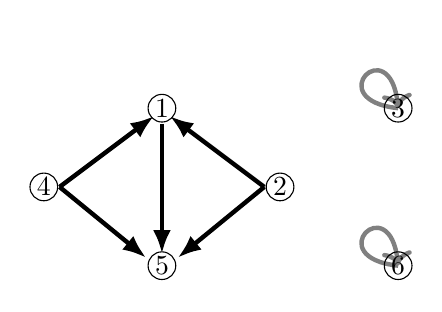
\begin{tikzpicture}
        \coordinate (A1) at (2, 2);
        \coordinate (A2) at (3.5, 1);
        \coordinate (A3) at (5, 2);
        \coordinate (A4) at (.5, 1);
        \coordinate (A5) at (2, 0);
        \coordinate (A6) at (5, 0);
        \draw[->,loop,min distance=1cm,in=96,out=174, ultra thick, gray] (A6) to (A6);
        \draw[->,loop,min distance=1cm,in=96,out=174, ultra thick, gray] (A3) to (A3);
        \draw[-{Latex[length=3mm]}, ultra thick] (2,1.8) -- (2,.15); 
        \draw[-{Latex[length=3mm]}, ultra thick] (.7,1) -- (1.9,1.9);
        \draw[-{Latex[length=3mm]}, ultra thick] (.7,1) -- (1.8,.1);
        \draw[-{Latex[length=3mm]}, ultra thick] (3.3,1) -- (2.1,1.9);
        \draw[-{Latex[length=3mm]}, ultra thick] (3.3, 1) -- (2.2,.1);
        \draw (A1) circle (0.5em) node{1};
        \draw (A2) circle (0.5em) node{2};
        \draw (A3) circle (0.5em) node{3};
        \draw (A4) circle (0.5em) node{4};
        \draw (A5) circle (0.5em) node{5};
        \draw (A6) circle (0.5em) node{6};
        \end{tikzpicture}
\end{multicols}
\end{itemize}
Which of the following statements are \textbf{true}?\\

\begin{choices}
\CorrectChoice $S$ is reflexive. %T
\choice $S$ is irreflexive. %F
\CorrectChoice $S$ is symmetric. %T
\choice $S$ is antisymmetric. %F
\choice $S$ is transitive. %F
%\choice $T$ is reflexive. %T
\choice $T$ is irreflexive. %F
\choice $T$ is symmetric. %F
%\choice $T$ is antisymmetric. %T
\CorrectChoice $T$ is transitive. %T
\choice None of the above
\end{choices}
%
\vfill


\end{parts}

%%%%%%%%%%%FREE RESPONSE%%%%%%%%%%%%

\newpage
\section*{Free Response/Proofs}
\noindent
\textbf{Show all work and justification.} Correct answer without justification receives no credit.
%%%%%%%%%%%%%%%%%%%%%%%%%%%%%%%
%%Boolean Algebra
\question[4] 
The operation $\uparrow$ is called the \textbf{Sheffer stroke} where $p \uparrow q \iff \neg(p\wedge q)$. 
Prove that $(p\uparrow p)\uparrow (q\uparrow q)$ is logically equivalent to $p\vee q$. 
\begin{solution}
 \begin{align*}
 (p\uparrow p)\uparrow (q\uparrow q) & = \neg[(\neg(p\wedge p))\wedge(\neg(q\wedge q))]\\
 & = (p\wedge p) \vee (q\wedge q)\\
 &= p\vee q.
 \end{align*}
\end{solution}

\newpage
%Counting
\question 4 different varieties of plant seeds are to be planted in a row. There are 15 varieties of vegetables and 10 varieties of flowers available. In each of the following cases, determine the number of possible arrangements of all the varieties of plant seeds under the given conditions.  For each part, you must give a brief justification in words (\textit{and optional diagrams}), and there is no need to give a numerical computation.
\begin{parts}
%%%
\part[3] Unrestricted.
\begin{solution}
 Since we are planting in a row and using different varieties, order matters and there is no repetition. Since we need 4 varieties to plant from  a choice of 25 varieties, there is a total of $(25)_4$ possible ways.
\end{solution}
\vfill
%%%
\part[3] Both the first and last positions are occupied by flowers.
\begin{solution}
 As mentioned in part a, we know this is represented by a list with no repetition. Since the first and fourth position needs to be flowers, there are 10 choices for the first position and 9 choices for the fourth position. Since there are no restrictions for the second and third position and we used up two of the available choices already, there are 23 and 22 choices for the second and third position, respectively. Then there is a total of $10\cdot 23\cdot22\cdot 9$ possible ways.
\end{solution}
\vfill

\part[3] All the vegetables are at one end of the row.
\begin{solution}
 In order for all vegetables to be grouped together at one end of the row, there can be either 0 vegetable, 1 vegetable, 2 vegetables, 3 vegetables, and 4 vegetables. Note that for the cases of 1 vegetable, 2 vegetables, and 3 vegetables, there are two ends of the row, so we would need to multiply by 2. So the total number of possible ways is sum of the cases of 0 vegetable, 4 vegetables, and twice the amount of having at one end of the row for the cases of 1 vegetable, 2 vegetables, and 3 vegetables:
 \[
1\cdot (10)_4 + (15)_4\cdot 1 + 2[ 15\cdot (10)_3 + (15)_2\cdot(10)_2 + (15)_3\cdot 10].
 \]
 
 Note that we still need to account for the order of the flower varieties.
\end{solution}
\vfill

%%%
\part[3] There must be more flowers than vegetables and order does not matter.
\begin{solution}
 Since we don't care about order, this is similar to counting sets. Then we have two cases: when we have 3 flowers and 1 vegetable, and 4 flowers and 0 vegetable. Then the total number of ways is 
 \[
 \binom{10}{3}\binom{15}{1} + \binom{10}{4}\cdot \binom{15}{0}
 \]
\end{solution}
\vfill



\end{parts}

\newpage
%Equivalence relations
\question Consider the following equivalence relation $\mathrel{R}$ on the Cartesian product $\R\times \R$.
\[
(a, b) \mathrel{R} (c, d) \iff \max(a, b)=\max(c, d)
\]
Here $\max$ is a function that returns the larger of two numbers. For example,
\begin{eqnarray*}
\max(9.3, -2) &=& 9.3\\
\max(-8, 2) &=& 2\\
\max(3, 3) &=& 3
\end{eqnarray*}

\begin{parts}
\part[4] Prove that $\mathrel{R}$ is transitive on the set $\R\times \R$ using the definition of transitive. 
\begin{solution}
Let $(a, b), (c, d), (e, f)\in \mathbb{R}\times\mathbb{R}$ such that $(a, b) \mathrel{R} (c, d)$ and $(c, d)  \mathrel{R} (e, f)$. Then $\max(a, b)=\max(c, d)$ and $\max(c, d) = \max(e, f)$. Since the $\max$ function outputs a real number, $\max(a, b)  = \max(e, f)$, which implies $(a, b)  \mathrel{R} (e, f)$. Therefore $ \mathrel{R}$ is transitive.
\end{solution}
\vfill

\part[2] If $X=(3, 2)$, list four elements of $[X]$ (the equivalence class of $X$) and describe the equivalence class.
\begin{solution}
 \begin{align*}
 [(3, 2)] & = \{ (3, 2), (0, 3), (3, -3), (2, 3), \dots \}\\
 &= \{(a, b) : (a=3, b<a) \vee (b=3, a<b)\}\\
 &= \text{ set of ordered pair of real numbers such that the largest of the two values is 3.}
 \end{align*}
\end{solution}
\vfill

\part[2] How many distinct equivalence classes are there for the relation $\mathrel{R}$ on the set $\R\times \R$? Briefly explain your reasoning.
\begin{solution}
 There are infinitely many equivalence classes since there are infinitely many real numbers that could be the maximum value in any order pair.
\end{solution}
\vfill

\end{parts}



\newpage
%%%Combinatorial proof
\question[8]
Prove the following statement {\bf combinatorially}. \textit{You may not modify the equation.}

Let $n$ and $k$ be natural numbers with $0\leq k<n$, then 
\[
\binom{n}{k+1} = \binom{k}{k} + \binom{k+1}{k} + \binom{k+2}{k} + \cdots + \binom{n-1}{k}.
\]

\begin{solution}
 Let $A = \{1, 2, 3, \dots, n\}$ for $n\in \mathbb{N}$. 
 
 \underline{Question:} How many possible subsets of $A$ with cardinality $k+1$ are there?
 
 \begin{itemize}
 \item[Answer 1:] Since we want all possible subsets of $A$ with cardinality $k+1$ and $|A|=n$, there are $\binom{n}{k+1}$ number of possible subsets.
 
 \item[Answer 2:] Let's look at all possible subsets of $A$ with cardinality $k+1$ where $i$ is the largest element. Since there are $k+1$ elements in each subset, we must have $k+1\leq i\leq n$. The remaining $k$ elements in the subset must all be less than or equal to $i-1$.  So there are $\binom{i-1}{k}$ possible choices.  The value of $i$ partitions the subsets into pairwise disjoint parts. So the total number of subsets is obtained by summing over all values of $i$. Then the total number of possible subsets is
 \[
 \displaystyle\sum_{i=k+1}^n \binom{i-1}{k} =  \binom{k}{k} + \binom{k+1}{k} + \binom{k+2}{k} + \cdots + \binom{n-1}{k}.
 \]
 
 Since Answer 1 and Answer 2 both answers the question, Answer 1 and Answer 2 are equal.
 \end{itemize}
\end{solution}


\end{questions}

%%%%%%%%%%%%%%%END-OF-FREE-RESPONSE%%%%%%%%%%%%%%%%%



%%%%%%%%%%%%%%%SCRAP%%%%%%%%%%%%%%%%%
%\newpage
%%Scrap
%\section*{Extra Paper}
%
\newpage
%\pagestyle{empty}
\section*{This page is intentionally left blank for computations!!!}

\newpage
\section*{This page is intentionally left blank for computations!!!}
%\newpage
%%\pagestyle{empty}
%\section*{This page is intentionally left blank for computations!!!}
%
%\newpage
%\section*{This page is intentionally left blank for computations!!!}
%%%%%%%%%%%%%%%SCRAP%%%%%%%%%%%%%%%%%

\end{document}  













